% TODOS:
% - 0.5 pt first page
% - where to introduce \coderef
% - ask nicolas if he understands BA overlapping 
% - general shortening
% - heuristic of kp_critical description 

%%%%%%%%%%%%%%%%%%%%%%%%%%%%%%%%%%%%%%%%%%%%%%%%%%%%%%%%%%%%%%%%%%%%%
% LaTeX Template: Project Titlepage Modified (v 0.1) by rcx
%
% Original Source: http://www.howtotex.com
% Date: February 2014
% 
% This is a title page template which be used for articles & reports.
% 
% This is the modified version of the original Latex template from
% aforementioned website.
% 
%%%%%%%%%%%%%%%%%%%%%%%%%%%%%%%%%%%%%%%%%%%%%%%%%%%%%%%%%%%%%%%%%%%%%

\documentclass[12pt]{report}
\usepackage[a4paper]{geometry}
\usepackage[myheadings]{fullpage}
\usepackage{fancyhdr}
\usepackage{lastpage}
\usepackage{amsmath} 
\usepackage{float} 
\usepackage{graphicx, wrapfig, subcaption, setspace, booktabs}
\usepackage[T1]{fontenc}
\usepackage[font=small, labelfont=bf]{caption}
\usepackage{fourier}
\usepackage[protrusion=true, expansion=true]{microtype}
\usepackage[english]{babel}
\usepackage{sectsty}
\usepackage{url, lipsum}
\usepackage[utf8]{inputenc}
\usepackage{titlesec}
\usepackage[T1]{fontenc}
%\usepackage{lmodern}
\usepackage{pdfpages}
\usepackage{enumitem}
\usepackage{tabularx}
\usepackage{subfig}

\onehalfspacing
\setcounter{tocdepth}{5}
\setcounter{secnumdepth}{5}
\setlength{\parindent}{0pt}


%-------------------------------------------------------------------------------
% HEADER & FOOTER
%-------------------------------------------------------------------------------
\pagestyle{fancy}
\fancyhf{}
\setlength\headheight{15pt}
\lhead{Project Report}
\rhead{D. Gehrig, R.Theiler, N. Küchler, C. Halter}
\rfoot{Page \thepage\ of \pageref{LastPage}}
	
\fancypagestyle{plain}{%
\fancyhf{}
\setlength\headheight{15pt}
\lhead{VO Project Report}
\rhead{D. Gehrig, R.Theiler, N. Küchler, C. Halter}
\rfoot{Page \thepage\ of \pageref{LastPage}}
}

%-------------------------------------------------------------------------------
% TITLE PAGE
%-------------------------------------------------------------------------------

\begin{document}

\title{ \normalsize \textsc{Vision Algorithms for Mobile Robotics - HS 2016}
\\ [2.0cm]
\HRule{0.5pt} \\
\LARGE \textbf{\uppercase{VO Project Report}}
\HRule{2pt} \\ [0.5cm]
%\normalsize \today \vspace*{5\baselineskip}
}

\author{
Daniel Gehrig: 12-922-738 \\
Raffael Theiler: 10-928-893 \\
Nicolas Küchler: 14-712-129 \\
Cyrill Halter: 13-928-171 }
\date{}

\maketitle
\tableofcontents
\newpage

%-------------------------------------------------------------------------------
% Section & chapter title formatting
%-------------------------------------------------------------------------------
\sectionfont{\scshape}
\titleformat{\chapter}{\normalfont\huge}{\thechapter.}{20pt}{\huge}
\titlespacing*{\chapter}{0pt}{-20pt}{30pt}

%-------------------------------------------------------------------------------
% BODY
% how to use this template:
% - write into the module corresponding to the topic you are working on
% - start a new section for each subtask
%
% - add your matriculation number in the author part of the title
%-------------------------------------------------------------------------------

%-------------------------------------------------------------------------------
% Parameter values
%-------------------------------------------------------------------------------
% VO + BA
\def \criticalKpBA {50\,}
\def \trackerMaxBidirectionalErrorBA {2.1\,}
\def \ransacNumIterationsBA {2000\,}
\def \baEveryNthFrame {4\,} 
\def \baReplace {6\,}
\def \baReplaceframes{6\,} %TODO : DANIEL FIX THIS

% VO
\def \harrisPatchSize {9\,}
\def \harrisKappa {0.08\,}
\def \numKeypoints {800\,}
\def \nonmaximumSupressionRadius {10\,}
\def \descriptorRadius {13\,}
\def \matchLambda {8\,}
\def \triangulationAngleThreshold {3\,}
\def \candidateCap {500\,}
\def \addCandidateEachFrame {100\,}
\def \triangulationMaxReprError {20\,}
\def \criticalKp {0\,}
\def \trackerMaxBidirectionalError {infinity\,}
\def \trackerBlocksize {13\,}
\def \ransacNumIterations {500\,}
\def \ransacPixelTolerance {10\,}

\newcommand{\coderef}[1]{[$\square$\kern-0.78em{$\equiv$}\:#1]\:}

\chapter{Introduction}
\vspace{-10mm}
\section{Monocular Visual Odometry}
The following report describes a completely monocular visual odometry (VO) pipeline. It relies on the input of a single camera feed to estimate a trajectory which is valid up to an unknown scale factor.

\section{Parameter Settings}
\label{params}
Before starting our VO pipeline by executing the file \emph{main.m}, the tester has to choose the data set, whether or not bundle adjusted and/or trajectory alignment to the ground truth should be performed. The last two are controlled with variables \emph{align\_to\_ground\_truth} and \emph{bundle\_adjustment} while the first can be used to distinguish between the KITTI (ds=0), Malaga (ds=1), Parking (ds=2) and our own (ds=3) data set. (\ref{dataset})

\section{Additional Work}
The successful implementation of the VO pipeline involved the tuning of several parameters which were vital to the stable performance. This was done by performing a quantitative simulation in order to find the combination that leads to the best trajectory estimate. For this a performance metric consisting of the average trajectory deviation was defined and used to simulate several combinations of the parameters. More on this analysis can be found in section \ref{simulation}. \par
For the purpose of testing these ideal parameters we recorded an own video and integrated it into the existing VO pipeline. This is an important test, because it assured us that we were not over-fitting our parameters to the benchmark data sets. More information on the data set can be found in section \ref{dataset}. \par
Unfortunately scale drift is inevitable in a VO pipeline due to errors in the pose and landmark estimates. To combat this drift multiple views can be refined using bundle adjustment (BA). We integrated a form of sliding window and overlapping bundle adjustment into the existing pipeline in order to refine both structure and motion. The adjusted estimates are significantly more accurate but at the cost of computational performance. For further information consult section \ref{bundle adjustment}.

\chapter{Functionality}
The following points summarize the pipeline's functionality. 
Topics that are documented further in the code will be denoted by \coderef{filename} with the respective file name.

\section{Bootstrapping}
To initialize the pipeline, an initial point cloud is triangulated between two key frames (frame 1 and 3) and the respective camera homographies are estimated. 
Using the \emph{Harris corner detector}, key points are extracted from images 1 and 3 and matched (using the SSD of the corresponding descriptor patches).
In the following step, the camera homography of frame 3 is estimated by calculating and decomposing the essential matrix using the \emph{eight-point algorithm} (since K is known). 
For robustness, \emph{RANSAC} is performed with a reprojection error tolerance of \ransacPixelTolerance and \ransacNumIterations iterations. 
The resulting inliers are then used to calculate the final landmarks and pose \coderef{initializePointCloudMono.m}.      

\section{Frame Processing}
Subsequent frames are processed in a Markovian fashion, meaning that information from the previous frame is sufficient to compute all necessary variables of the next frame \coderef{processFrame.m}. \par
When processing a new frame, first key points (matched with landmarks) are tracked from the previous image to the next image using the MATLAB implementation of a \emph{Kanade-Lucas-Tomasi tracker (KLT)} \coderef{propagageState.m}. 
Due to the large displacement of key points across images, 3 pyramidal levels and a patch size of \trackerBlocksize x \trackerBlocksize pixels are used. \par
In a second step the new camera homography is computed using the new 2D-3D correspondences between matched key points and landmarks. 
This can be computed efficiently using the \emph{P3P algorithm} in conjunction with \emph{RANSAC} \coderef{localizationRANSAC.m}. 
Using only three points allows for few iteration cycles (\ransacNumIterations cycles with a pixel tolerance of \ransacPixelTolerance). 
Outliers and key points that are discarded by the \emph{KLT} tracker are removed together with their corresponding landmarks.\par

Next, new landmarks are triangulated from candidate key point tracks which have been tracked over several frames. 
Tracks are discarded if they are lost by the \emph{KLT} tracker.
Triangulation is performed between the track end point and start point. 
New landmarks are triangulated asynchronously as soon as the angle between the bearing vectors at the track start point and end point exceeds \triangulationAngleThreshold degrees. 
New landmarks are discarded if their reprojection error exceeds \triangulationMaxReprError pixels or if they are triangulated behind the camera \coderef{tryTriangulate.m}. \par 
This candidate loss through tracking and triangulation means that new candidate key points must be added continuously. 
\addCandidateEachFrame new candidate key points are extracted from each frame using a Harris corner detector. 
To achieve a more robust behavior, the \emph{Harris score} is suppressed around existing candidate key points before feature extraction \coderef{suppressExistingMatches.m}. This ensures that the same key points are not added multiple times and enables a more uniform distribution of key points across the frame. 
In order to make our VO pipeline more robust to scale drift, we added an adaptive bearing angle threshold that depends on the number of currently matched key points and defines the angle necessary for candidates to be added as key points, the threshold being lower wen less key points are currently active.
\chapter{Additional Features}
\section{Data Set}
\label{dataset}

\section{Bundle Adjustment}
\label{bundle adjustment}
As mentioned in section ?? the stand-alone VO pipeline suffers from a significant amount of scale drift. This means that over the trajectory, the average scale of the displacements changes. \par
To counteract this drift, it is possible to use bundle adjustment (BA) which minimizes the reprojection error of landmarks over several views. In the pipeline, windowed BA is implemented. Every ?? frames, keypoints are adjusted and replaced over the last ?? frames. In order to ensure continuity, the adjusted point cloud and trajectory is translated such that the second last position (????? the second to last location??????) of the last segment coincides with first position of the newly adjusted segment. \par
Using BA, scale drift can be effectively counteracted as Fig. ?? a and b show. \par
Advantageous as BA in its current form may be, it is also very slow. This can be attributed to the fact that there are too many landmarks and poses for too few observations. In this case the Levenberg Marquart Optimization algorithm must be used leading to very poor performance. A way to improve this is to tune the tracking and triangulation parameters in a way to lose minimal matches over successive frames. This ensures that key points are observed several times before BA is executed. 

\section{Ground Truth Alignment and Error Analysis}
\label{simulation}

For a stable operation of the VO pipeline, optimized parameters must be chosen to control detection and matching of new key points, triangulation etc. To determine the optimal parameters, a suitable cost function must be defined to determine the quality of the resulting trajectories. To this end it is reasonable to compare the total error resulting after aligning the trajectory to the ground truth using the following formula:
\begin{equation}e_p = \underset{R,t,s}{\min} \sum_i (sR \cdot p_{GT, i} + t - p_{est, i})^2\end{equation}
$$e_r = \sum_i rotMatToRotVec(R^* \cdot R_{est,i} \cdot R_{GT, i}^T)^2$$
Where i is the index along the trajectory, $e_p$ is the positional error, $e_r$ is the rotational error, $p_{GT}$ and $R_{GT}$ are the ground truth position and rotation, $p_{est}$ and $R_{est}$ are the estimated position and rotation and $R^*$ is the argument for R when $e_p$ is minimal. The function rotMatToRotVec transforms the rotation matrix into a rotation vector of the form $\phi = \theta n$  Using these error metrics a detailed error analysis over the first ?? frames was done. More information on this can be found in section ??.


\chapter{Performance}
\label{performance}

\section{Error Analysis of Params}

In order to do a thorough optimization, a total of 15 parameters would have to be varied simultaneously. 
Brief descriptions of these parameters can be found in \emph{parameters.txt} \coderef{parameters.txt}.
Such a large number of variables, however, leads to an intractable search space for optimization. 
To curb the computational burden we segmented parameter selection into a preliminary simulation step \coderef{simTaskScheduler.m} which identified sensitive and non-sensitive parameters and a fine tuning step which investigated these parameters further. 
During the analysis the following error metrics were used to compare trajectories.

\begin{equation*}LE = \underset{R,t,s}{\min} \sum_i (s R \cdot p_{est, i} + t - p_{GT, i})^2\end{equation*}
\begin{equation*}OE = \sum_i \text{rotMatToRotVec}(R^* \cdot R_{est,i} \cdot R_{GT, i}^T)^2\end{equation*}

Where $i$ is the index along the trajectory, $LE$ is the location error, $OE$ is the orientation error, $p_{GT}$ and $R_{GT}$ are the ground truth location and orientation, $p_{est}$ and $R_{est}$ are the estimated location and orientation and $R^*$ is the argument for R when $LE$ is minimal. 
The parameters $s$, $R$ and $t$ describe a generic similarity transformation. 
The function \emph{rotMatToRotVec} transforms the rotation matrix into a rotation vector of the form $\phi = \theta n$ \coderef{rotMatToRotVec.m}.

\section{Preliminary Simulations}

First, a sensible parameter configuration was guessed for each cluster. 
Then groups were fine tuned either manually or using simulation.  
Parameters which showed an increase in accuracy (deviation from ground truth, see chapter \ref{simulation}) and robustness (successful completion of run with varying other parameters) were selected at each step.

\medskip

Good Harris parameters (patch size = 9 and $\kappa$ =  0.08) where identified with low tracking loss. 
Moreover, the maximal number of candidates was determined to have low impact above 500. 
The sensitive parameters and ranges were narrowed down to 5 and are presented in table \ref{table:significant-param-tuning}.

\subsection{Parameter Fine Tuning}  

In this step the above parameters were varied in their ranges, while the other parameters were held constant and the OE and LE were recorded. 
1000 different combinations were tested in total and their results are shown in an error histogram in figure \ref{fig:error_histogram}. 
While the LE exhibits a large variance, the orientation error is much more concentrated in one peak. 
This shows that the location error is influenced much more by the variation of our parameters so from here on only the LE will be discussed.
In table \ref{table:significant-param-tuning} the three parameter combinations that lead to the lowest LE can be seen. \par
To compare the robustness of these candidates it is necessary to see how well the algorithm performs for similar parameter combinations. 
For this purpose histograms showing the distribution of the 10 best and 200 best results for each parameter were constructed and are shown in figure \ref{fig:best10} and \ref{fig:best200}.
It can be seen that \emph{triangulate\_max\_repr\_error} is very robust as 50\% (5 out of 10) of the top 10 share this value. 
It therefore makes sense that all top 3 candidates share this value. 
Also with \emph{nonmaximum\_suppression\_radius} all top 3 share parameters with the majorities from the top 10. 
This trend is supported further by the top 200 histograms.
The parameter \emph{tracker\_max\_bidirectional\_error} is shared by the top 3 and top 10. 
If we compare \emph{critical\_kp} we see that although two of the top three share the same value as the majority in the top 10 the best value is reached with a value of 100.
This can be explained by the fact that in the KITTI data set the second curve contains a dark patch which makes it hard to track key points. 
If there is no safety net many runs will just fail because they have too few landmarks to perform localization. 
A histogram displaying all failed runs illustrates this point in figure  \ref{fig:exceptions}. 
It shows that a parameter value of 0 leads to the majority of the exceptions which leads us to believe that this value is not robust although it may be optimal. 
The final parameter is \emph{add\_candidate\_each\_frame} which is robust to failure for all top 3 although not optimal for the best candidate.

\medskip

Factoring in all available information, we arrived at the parameter configuration described in table \ref{table:significant-param-tuning} under \emph{Chosen}.

\begin{table}[htp]
	\centering
	\caption{Parameter Fine Tuning: best three parameter combinations and their respective location error (LE). $LE_{max}$ : 23187, $LE_{min}$: 6664.9}
	\label{table:significant-param-tuning}
	\begin{tabular}{lrrrrr}
		\hline
		\textbf{Parameters}                &         \textbf{Range} & \textbf{Best} & \textbf{2nd Best} & \textbf{3rd Best} & \textbf{Chosen} \\ \hline
		$LE$                &                        &          6664 &              6987 &              7207 &  \\ \hline\hline
		nonmaximum\_supression\_radius     &                10:2:16 &            12 &                10 &                10 & 10\\ \hline
		add\_candidate\_each\_frame        &              50:50:200 &           150 &               200 &               200 & 150\\ \hline
		triangulate\_max\_repr\_error      & [0.5, 1, 2, 5, 10, 20] &             5 &                 5 &                 5 & 5\\ \hline
		critical\_kp                       &       [0, 20, 50, 100] &           100 &                 0 &                 0 & 100\\ \hline
		tracker\_max\_bidirectional\_error &      [2.1, 5, 9999999] &             5 &               2,1 &                 5 & 5\\ \hline
	\end{tabular}
\end{table}

\begin{figure}[htp]
	\centering
	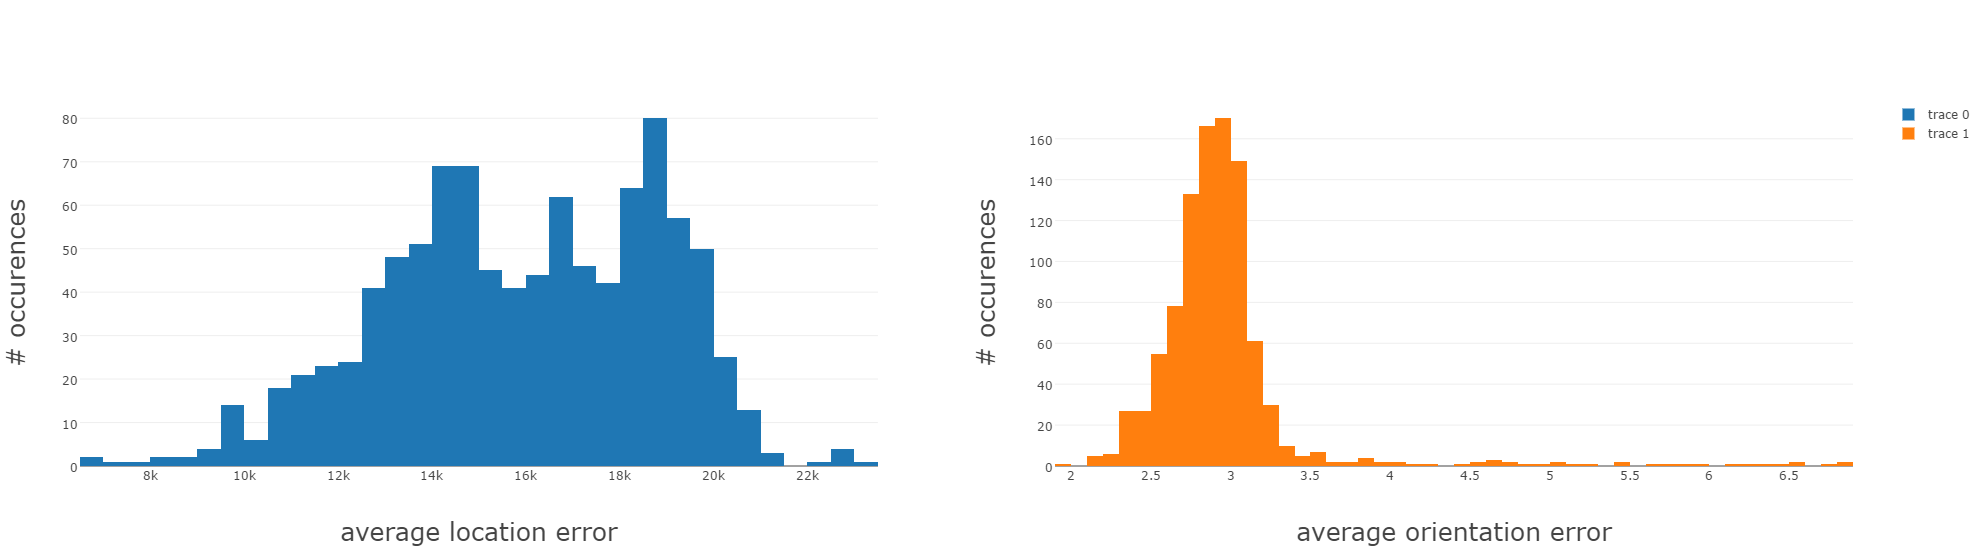
\includegraphics[width=1\textwidth]{figures/error_histogram}
	\caption{Distribution of the location error $LE$ and orientation error $OE$. 
	An outlier (23.79) was removed from the orientation errors. 
		$OE_{min}: 1.97$, 
		$OE_{max}: 23.79$,
		$OE_{med}: 2.89$,
		$LE_{min}: 6664.9$,
		$LE_{max}: 23187.5$,
		$LE_{med}: 16059.0$}
	\label{fig:error_histogram}
\end{figure}

\begin{figure}[htp]
	\centering
	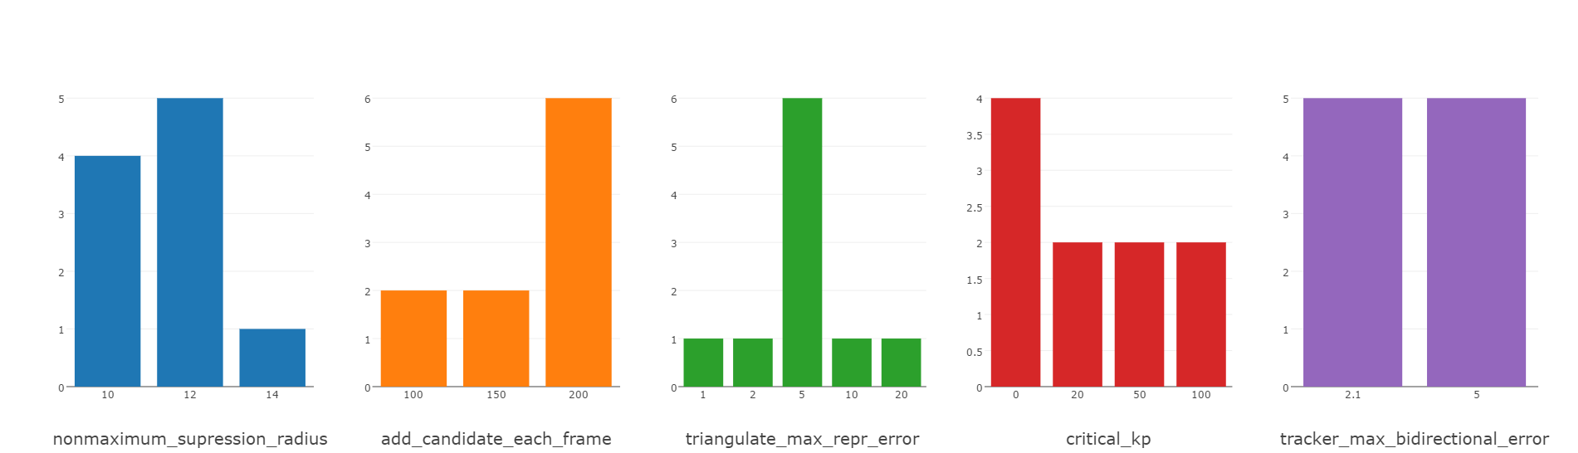
\includegraphics[width=1\textwidth]{figures/best10}
	\caption{Parameter distribution of the best 10 results  (15\% of the dynamic range).}
	\label{fig:best10}
\end{figure}

\begin{figure}[htp]
	\centering
	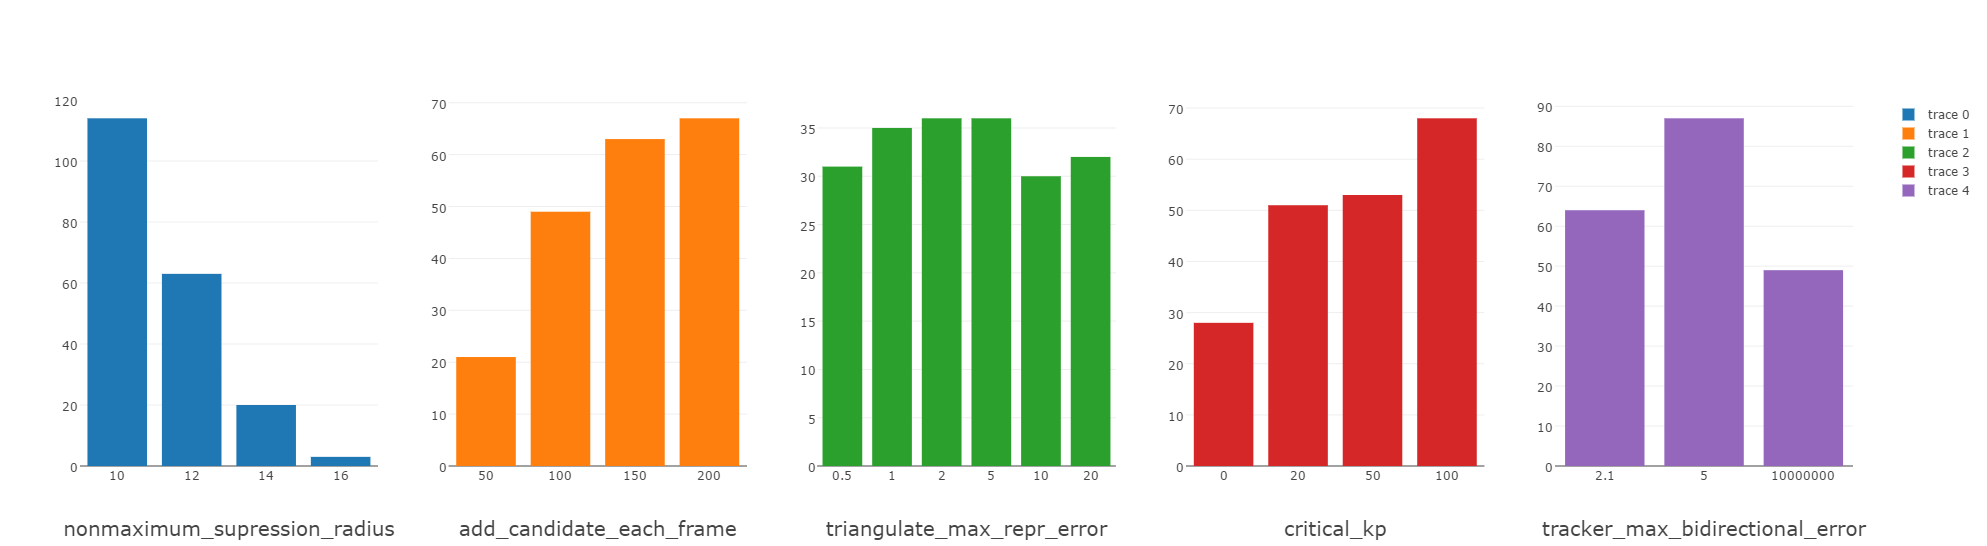
\includegraphics[width=1\textwidth]{figures/best200}
	\caption{Parameter distribution of the best 200 results  (40\% of the dynamic range).}
	\label{fig:best200}
\end{figure}

\begin{figure}[htp]
	\centering
	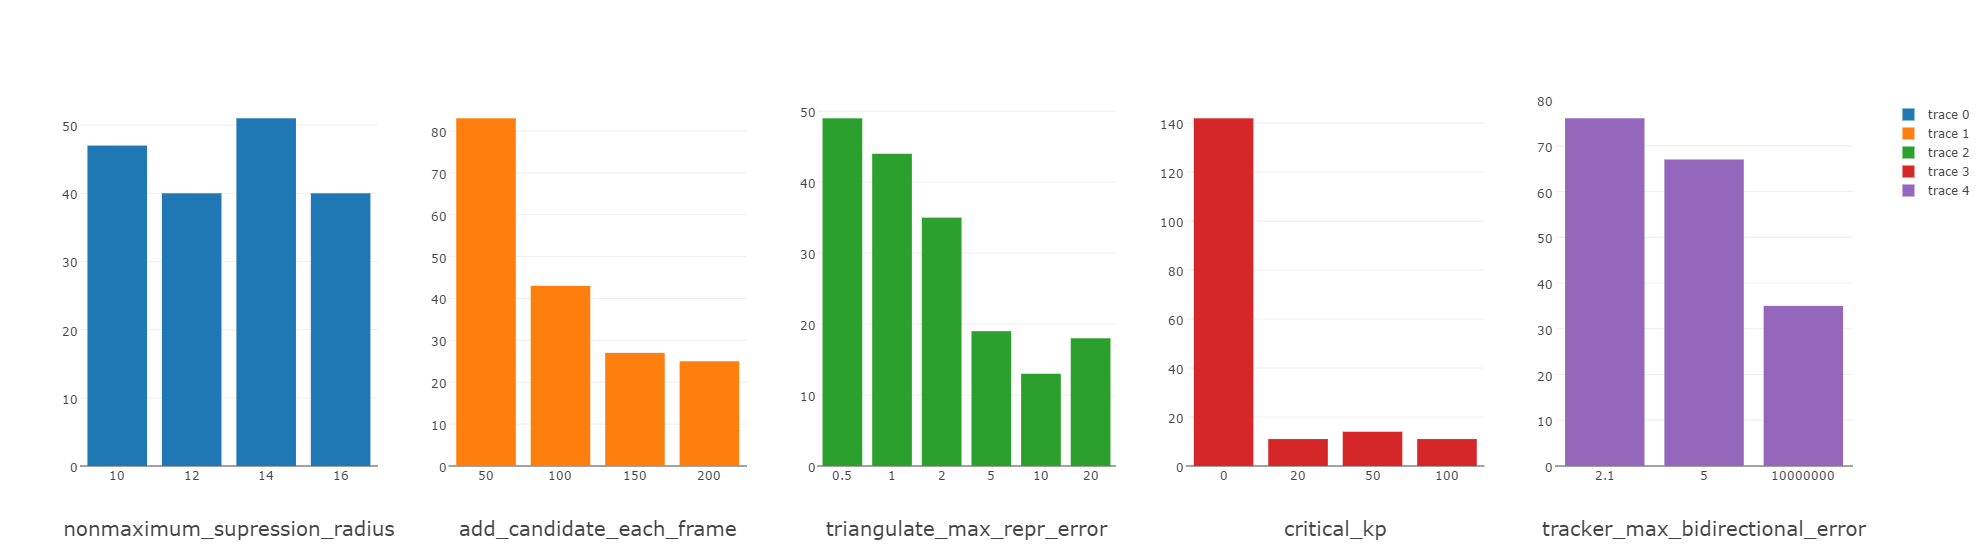
\includegraphics[width=1\textwidth]{figures/exceptions}
	\caption{Parameter distribution of all runs that terminated due to excessive loss of key points. }
	\label{fig:exceptions}
\end{figure}
\chapter{Appendix}

\end{document}

%----------------------------------V., 2007. Oxidants in Chronficacy of lazarois and my3. \textit{Toxic Neuropathy Clinical Presentation.} [--------------------------------

%\begin{figure}[!ht]
%	\centering
%	\includegraphics[width=0.8\textwidth]{file_name}
%	\caption{
%	\centering
%	\label{label:file_name}
%\end{figure}

%\begin{figure}[!ht]
%	\centering
%	\includegraphics[width=0.8\textwidth]{graph}
%	\caption{Blood pressure ranges and associated level of hypertension (American Heart Association, 2013).}
%	\centering
%	\label{label:graph}
%\end{figure}

%\begin{wrapfigure}{r}{0.30\textwidth}
%	\vspace{-40pt}
%	\begin{center}
%		\includegraphics[width=0.29\textwidth]{file_name}
%	\end{center}
%	\vspace{-20pt}
%	\caption{
%	\label{label:file_name}
%\end{wrapfigure}

%\begin{wrapfigure}{r}{0.45\textwidth}
%	\begin{center}
%		\includegraphics[width=0.29\textwidth]{manometer}
%	\end{center}
%	\caption{Aneroid sphygmomanometer with stethoscope (Medicalexpo, 2012).}
%	\label{label:manometer}
%\end{wrapfigure}

%\begin{table}[!ht]\footnotesize
%	\centering
%	\begin{tabular}{cccccc}
%	\toprule
%	\multicolumn{2}{c} {Pearson's correlation test} & \multicolumn{4}{c} {Independent t-test} \\
%	\midrule	
%	\multicolumn{2}{c} {Gender} & \multicolumn{2}{c} {Activity level} & \multicolumn{2}{c} {Gender} \\
%	\midrule
%	Males & Females & 1st level & 6th level & Males & Females \\
%	\midrule
%	\multicolumn{2}{c} {BMI vs. SP} & \multicolumn{2}{c} {Systolic pressure} & \multicolumn{2}{c} {Systolic Pressure} \\
%	\multicolumn{2}{c} {BMI vs. DP} & \multicolumn{2}{c} {Diastolic pressure} & \multicolumn{2}{c} {Diastolic pressure} \\
%	\multicolumn{2}{c} {BMI vs. MAP} & \multicolumn{2}{c} {MAP} & \multicolumn{2}{c} {MAP} \\
%	\multicolumn{2}{c} {W:H ratio vs. SP} & \multicolumn{2}{c} {BMI} & \multicolumn{2}{c} {BMI} \\
%	\multicolumn{2}{c} {W:H ratio vs. DP} & \multicolumn{2}{c} {W:H ratio} & \multicolumn{2}{c} {W:H ratio} \\
%	\multicolumn{2}{c} {W:H ratio vs. MAP} & \multicolumn{2}{c} {\% Body fat} & \multicolumn{2}{c} {\% Body fat} \\
%	\multicolumn{2}{c} { & \multicolumn{2}{c} {Height} & \multicolumn{2}{c} {Height} \\
%	\multicolumn{2}{c} { & \multicolumn{2}{c} {Weight} & \multicolumn{2}{c} {Weight} \\
%	\multicolumn{2}{c} { & \multicolumn{2}{c} {Heart rate} & \multicolumn{2}{c} {Heart rate} \\
%	\bottomrule
%	\end{tabular}
%	\caption{Parameters that were analysed and related statistical test performed for current study. BMI - body mass index; SP - systolic pressure; DP - diastolic pressure; MAP - mean arterial pressure; W:H ratio - waist to hip ratio.}
%	\label{label:tests}
%\end{table}}<++>}<++>}<++>}<++>}<++>}<++>}<++>